\chapter{Methodology of Proposed Work}
The work that we proposed here for navigating a robot using natural language based instruction has 3 major sections. They are:
\begin{itemize}
    \item Web Environment
    \item Dataset and the Model
    \item Map for Providing Output
\end{itemize}
Now we'll go through the elaboration of these sections. \\

\section{The Web Environment}
The main work that we've done to demonstrate our task is designing a web interface. Initially this runs inside local server but it could easily be deploy-able to actual web server. We design this web interface so that the module could easily be used in real life scenario.\\

An image of the designed interface is as follow. \\
\begin{figure}[h]
    \centering
    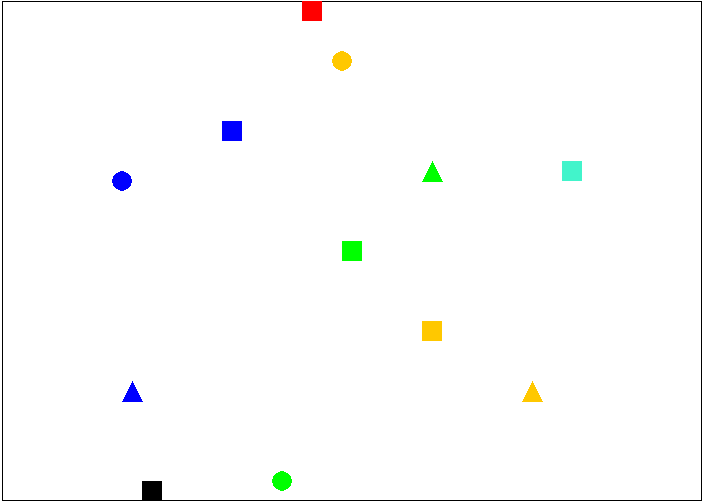
\includegraphics[scale=0.45]{environment}
    \caption{Used Web Interface}
\end{figure}
\vline

The functionality we added inside the interface is: \\
\begin{itemize}
    \item Taking voice input
    \item Converting voice to text
    \item Sending converted text to the model
    \item Showing output on map from the output of the model
\end{itemize}

Now we'll go through details of these functionalities. \\

\subsection{Taking Voice Input}
As we can see in the figure above, there are two buttons: `Record Start' and `Record End'. The name of the buttons describe the functionalities. If we click on the button `Record Start' then we go to the recording mode. After entering the recording mode we speak to the connected microphone and give navigation instruction in language that we use our day to day life. \\

There is no time limit added with voice input. It means as long as we want we can give instruction. What happened here is we basically record the voice which is spoken.


\subsection{Converting Voice to Text}
When our instruction ended, we will click on `Record End' button. After pressing the button the recording will stop which was started when we pressed `Record Start' button. After the audio recording ended, we saved the audio in WAV format. \\

Immediately we convert the audio to the text. For this conversion we used Google Cloud Speech-to-Text service. There are several other ways to convert the voice into text but we find Google's service more reliable and accurate. As converting voice to text is a huge task which takes much time and large dataset so that we didn't develop our own version of voice-to-text. Competing with Google's dataset and algorithm is also a great challenge. As our project is neither voice-to-text conversion focused so we used Google's service here.\\

After converting the audio to text, the converted text appeared in the text box in our interface. We kept the option to further modify the text. Though the converted voice mostly accurate but sometimes some Bengali names spoken in Bangladeshi accent becomes difficult to convert in English. If some words converted wrongly so that we can manually edit it for our navigation purpose.

% 1120193110500585

\subsection{Sending Converted Text to Model}
After conversion and/or necessary modification done, if we press the `Get Route' button, then the text is sent to the model which is already saved in local server. We trained the model previously and saved the tokenizer and the model in our server. Once we clicked on the button then the text is first tokenized and then applied on the model.

\subsection{Showing Output on the Map from the Output of the Model}
After applying the text on the model, the model gives us the list of the places sequentially that is said to be navigated in the text. Based on the places list, the required path is generated and shown on the map.


\section{Dataset and Model}
Dataset and Model are required for learning purpose. First have a look where and for what purpose we used learning. \\

As we said we'll navigate a robot using natural language instruction, so understand the natural language instruction we'll use machine learning method. So the basic question is, what was the main challenge we encounter so we pick the learning method? \\

As we want to enable our robot/agent to navigate according to natural language based instruction, so our robot/agent should have the ability to understand all kind of instruction. As instruction format could be different from person to person like some person may use complex sentence structure, some person may could use complex grammar or some person may could use very simple instruction. As we don't know how our input instruction would look like so that we can't use naive string matching type algorithm. \\

Lets consider an example. Lets we have an instruction: `Go to point A through point B'. In this instruction the robot has to go to point B first then point A. The same instruction could be in another format: `Go to point B first then go to point A'. The robot has to accomplish same task but it is given in different format. The given instruction could be even further complex where the robot may have to navigate through three or more points. If we try to implement a `rule based model' like if we got this type of sentence structure then we'll do this else we'll do something different, this type of approach will be very naive and difficult to implement. Furthermore, the robot won't have the capability to understand a new instruction what it never seen before. \\

So situation like described above need the approach of machine learning. So here instead of implementing rule based model we implemented a learning approach for robot navigation. \\

\subsection{Dataset}
As we've already described why we are using learning. For learning, we need a dataset. Here we'll look how we've designed our dataset. \\

We are navigating through 8 points on Dhaka University campus. This points are: Curzon Hall, Dr. Muhammad Shahidullah Hall, Amar Ekushey Hall, Fazlul Haque Muslim Hall, Bangla Academy, TSC, Shaheed Minar and Dhaka Medical College Hospital. So our navigation instruction will be based on these eight points. In other word, all of navigation instruction that we included in our dataset have at last one of these points. \\

As we'll look in next section, the model we used here is basically a classifier. The classifier will give us the place names and their order, which place have to navigate before which place.\\

Our dataset has nine columns. First column holds the instruction. The other eight columns are marked as: `place0' through `place7'. `place0' represent Curzon Hall. If we have Curzon Hall mentioned in the instruction the column `place0' will contain a value else it will contain a 0. If Curzon hall in mentioned in the instruction, according to the order, the `place0' column will contain a value. If the robot has to navigate Curzon Hall first among two other points then the row associated with the instruction will contain a value 3000. If Curzon Hall is the second point then the row has a value of 2000. If none of this true then the row will contain a value of 1000. \\

As we mentioned place0 holds values for Curzon Hall. Similarly place1 holds values for Dr. Muhammad Shahidullah Hall, place2 for Amar Ekushay Hall, place3 for Fazlul Haque Muslim Hall, place4 for TSC, place5 for Shaheed Minar, place6 for Bangla Academy and place7 holds values for Dhaka Medical College Hospital consecutively. \\

Here is a quick view of our dataset that we've used. \\

\begin{longtable}{|l|l|l|l|l|l|l|ll}
    \cline{1-7}
    instruction                                                                                           & place0 & place1 & place2 & place3 & place4 & place5 & place6 & place7 \\ \cline{1-7}
    \endfirsthead
    %
    \endhead
    %
    go to Dr. Muhammad Shahidullah Hall                                                                   & 0      & 1000   & 0      & 0      & 0      & 0      & 0      & 0      \\ \cline{1-7}
    start from Dr. Muhammad Shahidullah Hall to Shaheed Minar                                             & 0      & 2000   & 0      & 0      & 0      & 0      & 0      & 1000   \\ \cline{1-7}
    start journey from Bangla Academy to Dhaka Medical College Hospital via Dr. Muhammad Shahidullah Hall & 0      & 2000   & 0      & 0      & 3000   & 0      & 0      & 1000   \\ \cline{1-7}
    go from Dhaka Medical College Hospital to Amar Ekushey Hall                                           & 0      & 0      & 1000   & 0      & 0      & 0      & 0      & 2000   \\ \cline{1-7}
    go from Curzon Hall to Dhaka Medical College Hospital                                                 & 2000   & 0      & 0      & 0      & 0      & 0      & 0      & 0      \\ \cline{1-7}
\end{longtable}

\textbf{Data Preprocessing} \\
Before describing the model, we first need to prepare our data so that it can be fit to the model. \\

We used some cleaning operation they are: lowering the letters, removing unnecessary spacing, removing bad symbols like \# or \text{*} which has no purpose in navigation instruction. After that we make apply our instruction data to a Tokenizer. This tokenizer allows us to fit our text data to a trainable model. \\

When we evaluate our model or applying new data to our model, we do this same data preprocessing operation. \\


\subsection{Model}
The problem we are dealing with is basically a classification problem. As text is our training data so its better to use Sequential model here. Traditional neural network architecture is not suitable for our problem. In this problem we are dealing with text data. For text data, when we are processing a particular word we also have to recall previous words. Recognizing previous data in a traditional neural network is an impossible task.\\

As we are not dealing with image data so Convolutional Neural Network(CNN) is neither a good choice. For our intended task, neural network architecture of sequential model is the best choice. \\

After choosing sequential model as our classifier, now the question is what architecture of sequential model will we use? Should we use Recurrent Neural Network(RNN) or Long Short Term Memory(LSTM) architecture? First lets have a look on both of these architecture. \\

\textbf{Recurrent Neural Network(RNN)} \\
RNN is helpful to tackle problem when previous information also needed to consider for processing current information. RNN is an architechture of networks with loop. [Reference1] \\

The following figure shows a basic building block of RNN. \\

\begin{figure}[h]
    \centering
    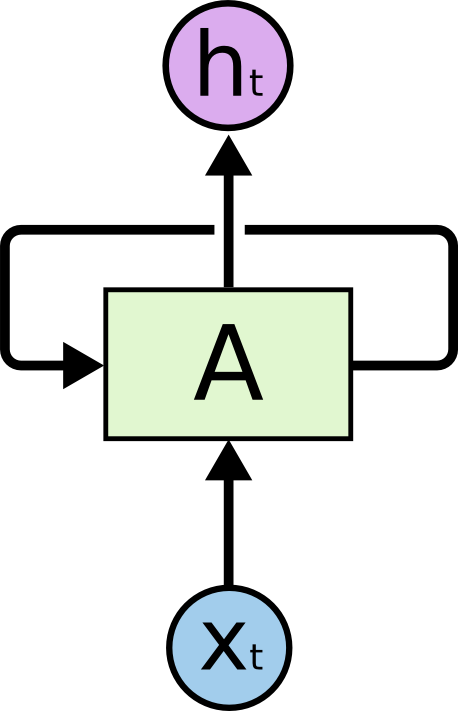
\includegraphics[scale=0.45]{rnn_single_block}
    \caption{Single Building Block of RNN[Reference2]}
\end{figure}
\vline

In the above figure, block $\textbf{A}$ represent a group of neural networks. It takes some input \textbf{$x_t$} and provide value \textbf{$h_t$} as output. \\

We can think RNN as same network with multiple copies, each of which passes a message to its successor. [Reference3]. If we unroll the RNN it will look like as bellow. \\

\begin{figure}[h]
    \centering
    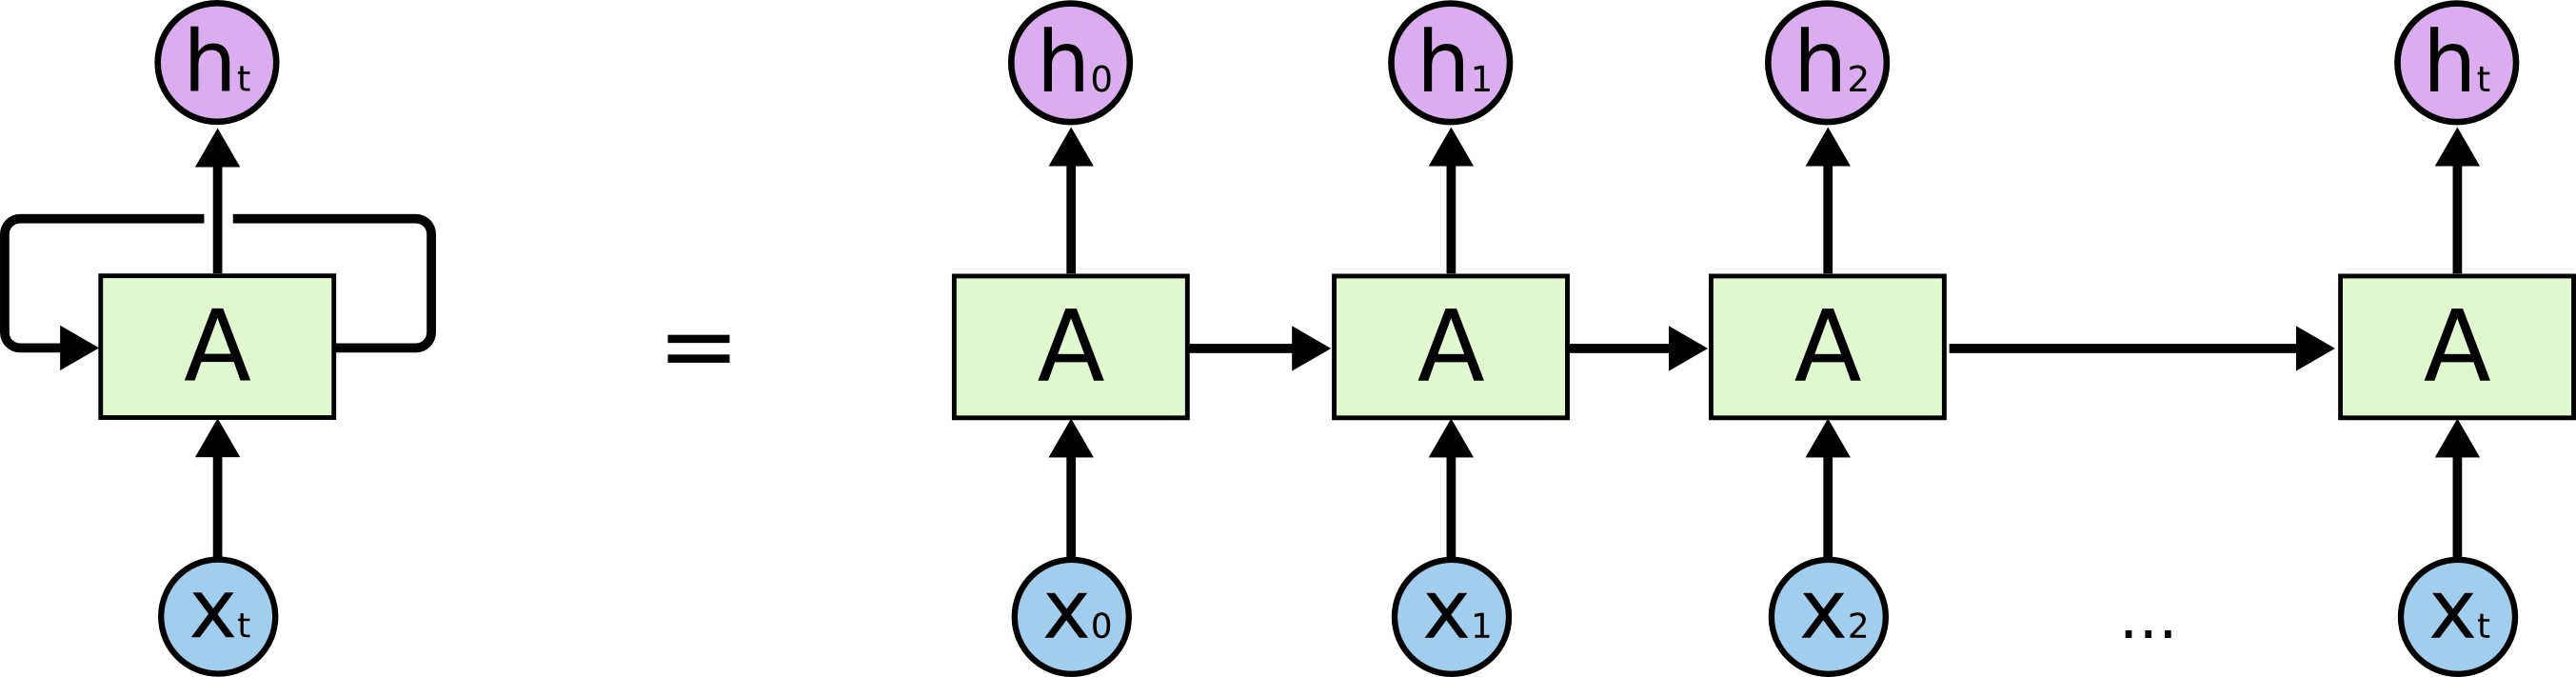
\includegraphics[scale=0.45]{rnn_unrolled}
    \caption{Unrolled RNN[Reference4]}
\end{figure}
\vline

Through previous year in research and industry RNN solved many exciting problems like speech recognition, image captioning, language modeling etc. But RNN has its limitation too. Long-term dependency is the problem that we encounter with RNN. Long-term dependency problem arises when a gap created between a relevant information and the place where it needed. Though theoretically RNN supposed not to have long-term dependency problem but practically it actually has. To solve the addressed problem, a special version of RNN, called LSTM is used. \\

For our problem that we are trying to solve, at first it seems that RNN is sufficient but soon we'll see LSTM provide us better result. \\

\textbf{Long Short Term Memory (LSTM)} \\
LSTMs are special structure of RNN which have the capability to learn long-term dependencies. Remembering an information which is may or may not be relevant for long period of is default behavior of LSTM networks. \\

In all type of RNNs, there is a chain of repeating modules. In a standard RNN, the repeating module have very simple structure like tanh layer. \\

\begin{figure}[h]
    \centering
    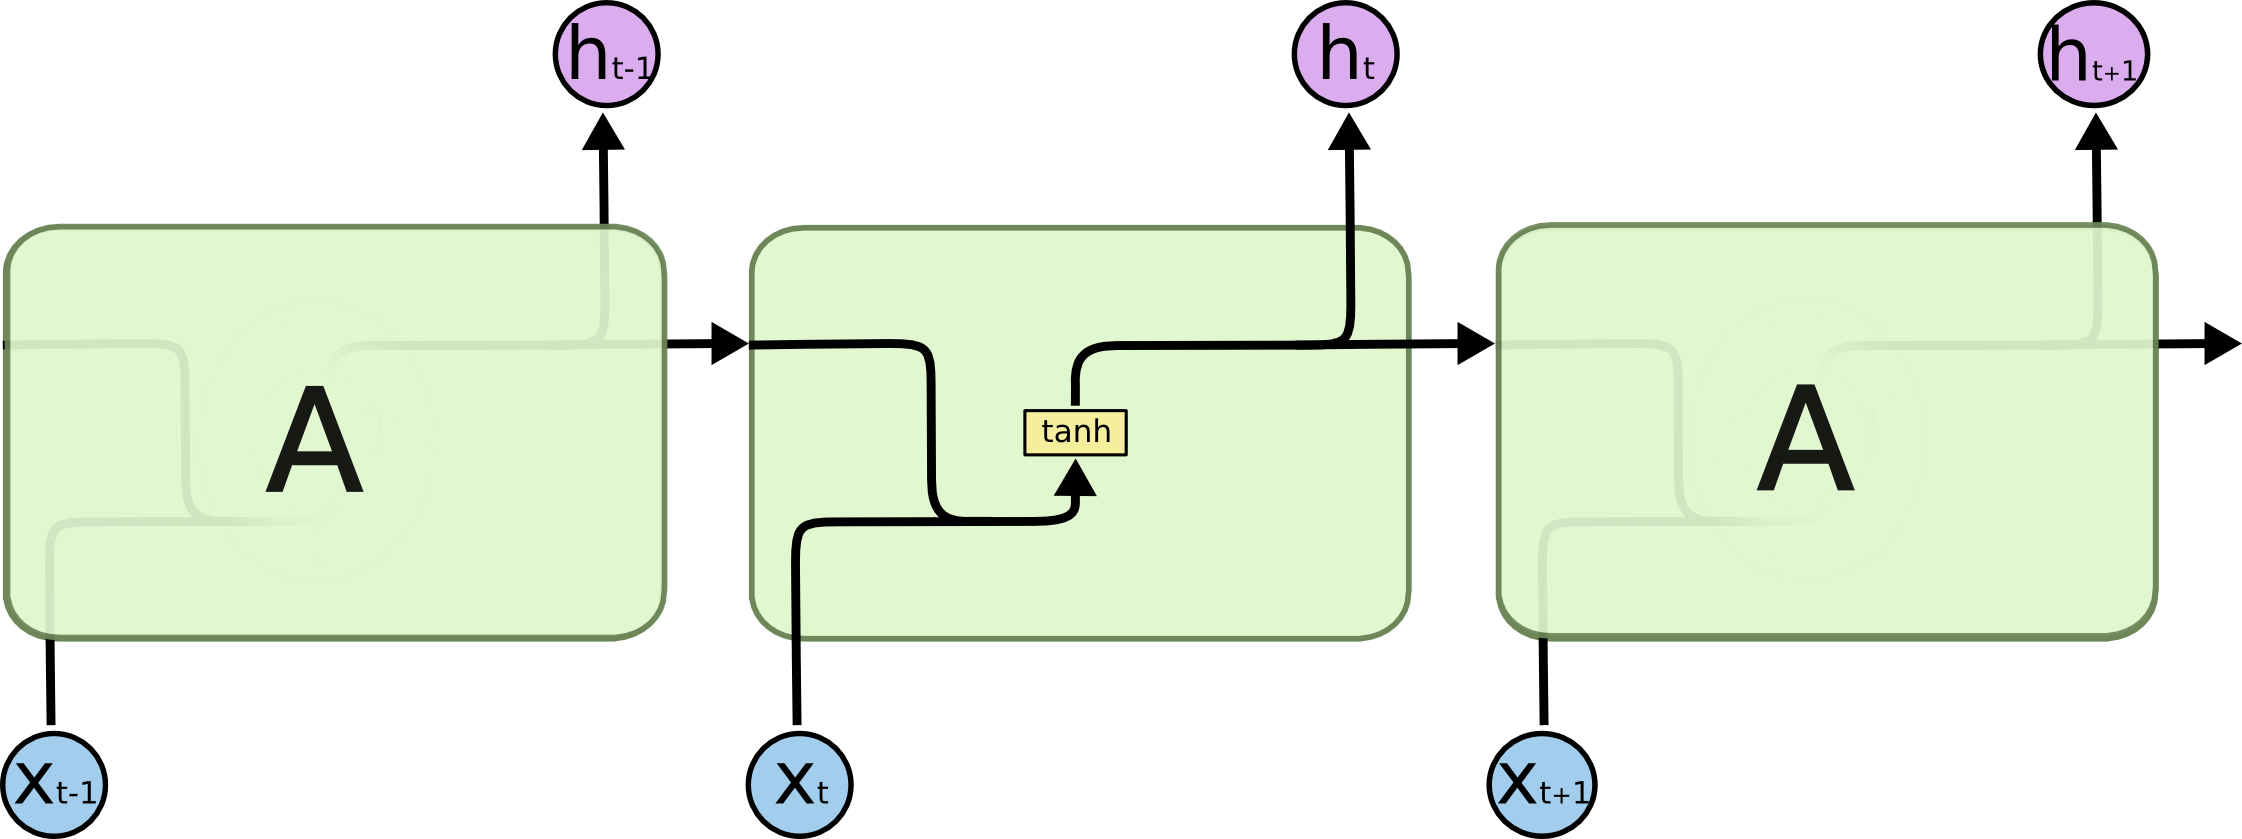
\includegraphics[scale=0.45]{repeating_rnn}
    \caption{Single Layer of RNN in Repeating Module[Reference 5]}
\end{figure}
\vline

LSTMs also have RNN like chain structure, but in repeating module of LSTM a different structure is used. Instead of a single NN(neural network) layer, four layers are used and they interact a very special way. The following figure shows repeating module of LSTM. \\

\begin{figure}[h]
    \centering
    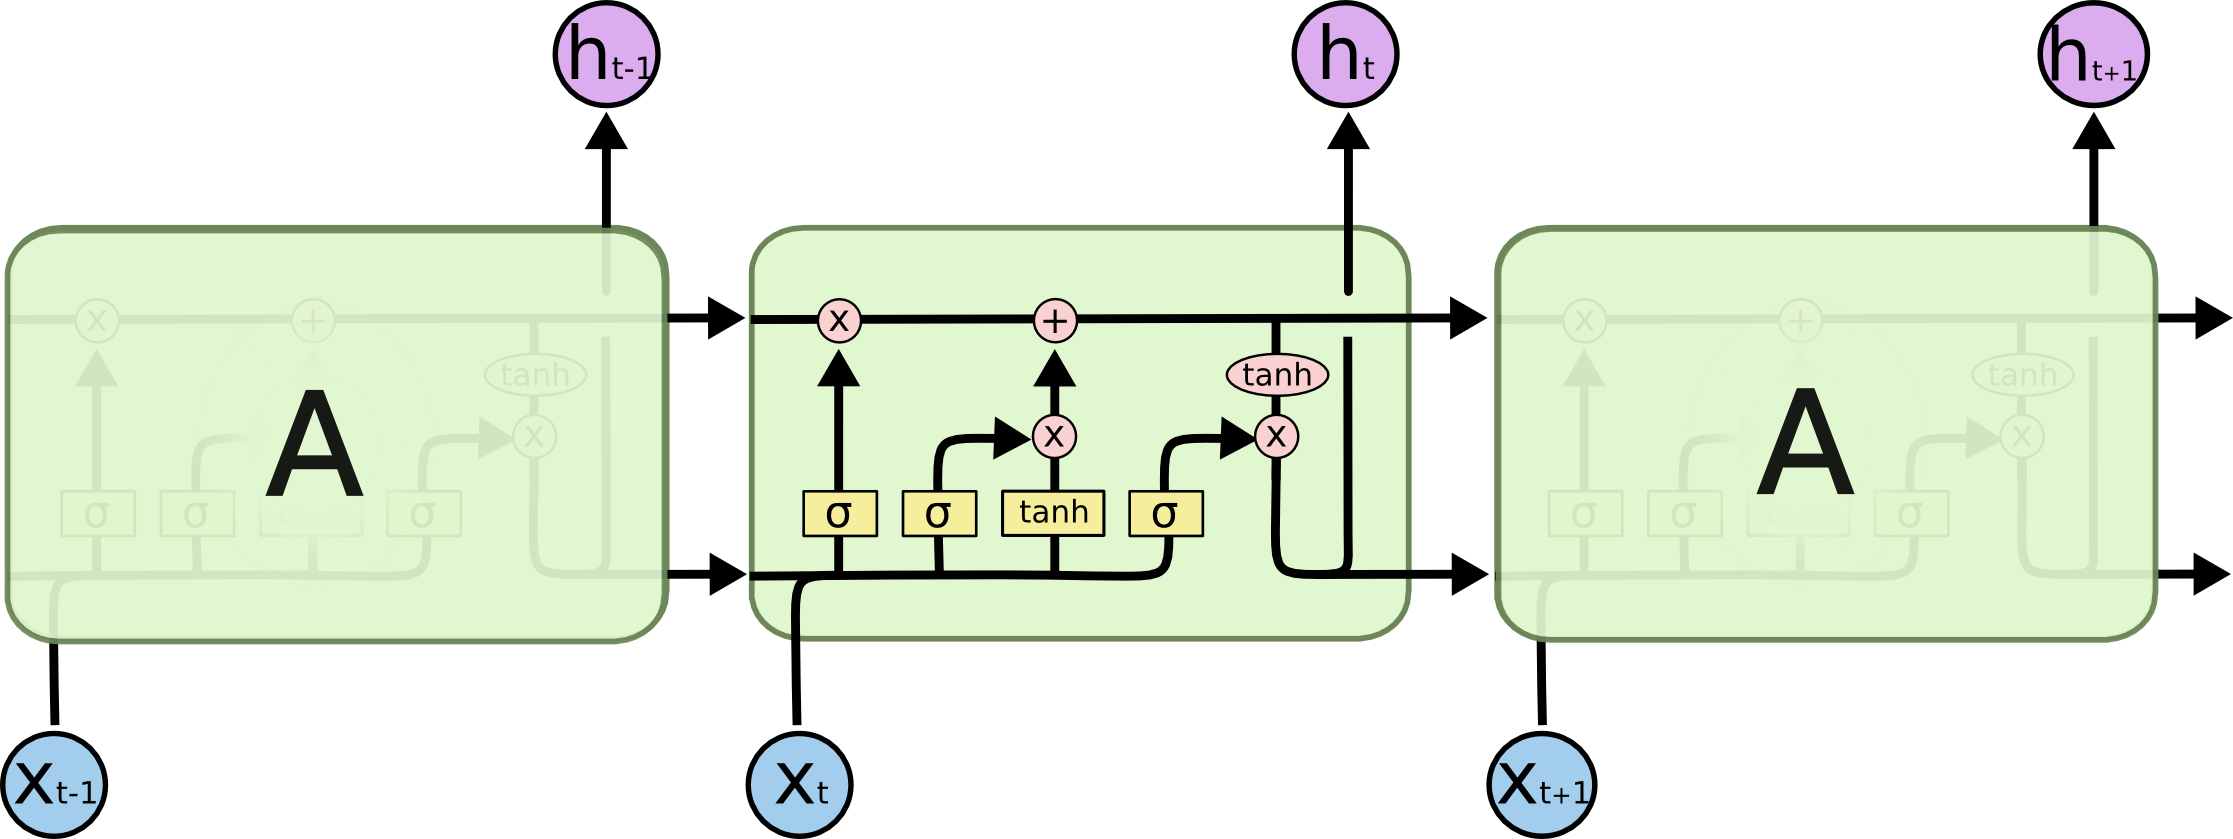
\includegraphics[scale=0.40]{repeating_lstm}
    \caption{Repeating LSTM module with Four Interacting Layers[Reference6]}
\end{figure}
\vline

Cell state is the key contributor of LSTM. Cell state works like kind of conveyor belt. This runs straight through the chain with only having some minor linear interaction. The LSTM posses the ability of adding or removing information to the cell state. This ability is carefully regulated by another structure called Gate. \\

Gates have the ability to modify the flow of information. Gates are composed of a sigmoid neural network layer and LSTM's pointwise multiplication operation. \\

\begin{figure}%
    \centering
    \subfloat[]{{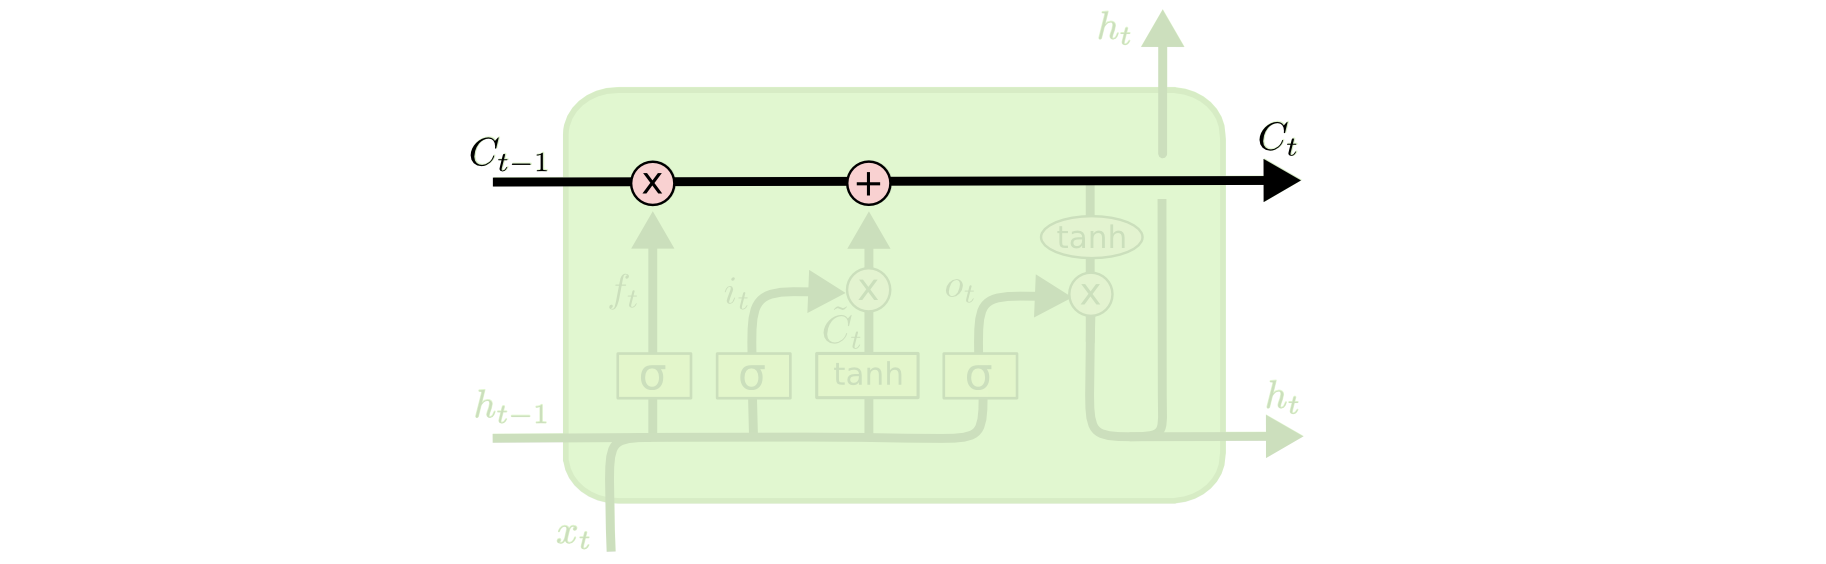
\includegraphics[scale=0.45]{cell_state_lstm} }}%
    \qquad
    \subfloat[]{{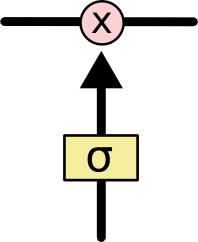
\includegraphics[scale=0.45]{lstm_gate} }}%
    \caption{LSTM's Cell State and Gate}%
    %\label{fig:example}
\end{figure}
\vline

The operations of LSTM are done in following three steps:
\begin{itemize}
    \item Forgettring unnecessary information from cell state
    \item Adding information to cell state
    \item Calculating output
\end{itemize}

For brevity we skip the details of each step. A full and quick overview of a LSTM cell can be easily understood from the figure below. \\

\begin{figure}[h]
    \centering
    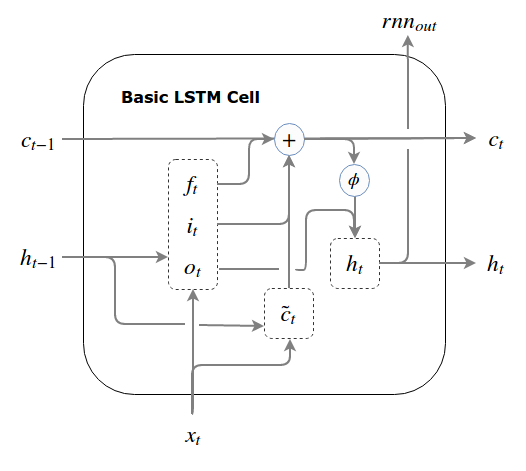
\includegraphics[scale=0.40]{lstm}
    \caption{Complete LSTM Cell[Reference7]}
\end{figure}
\vline


\subsection{Designed Architecture}		
As said earlier, we used LSTM for our classification task. We designed our architecture such a way, first we take s Sequential model. Then we add an Embedding layer with $30X100$ shape. After that We added a spatial dropout of 0.2. Then we add LSTM layer in our Sequential model with 128 hidden units and 0.2 recurrent dropout. At the end of the model, we added a Dense layer with 8 hidden units and we used $softmax$ as our activation function in the final Dense layer. \\

At the end of our model, we calculate loss using `categorical cross entropy'. We used $adam$ optimizer. Finally we select `accuray' as our metric of the model. \\

A quick view of our model is as follow. \\

\begin{table}[]
    \centering
    \begin{tabular}{|l|l|}
        \hline
        Layer             & Output Shape \\ \hline
        Embedding         & (30, 100)    \\ \hline
        Spatial (Dropout) & (30, 100)    \\ \hline
        LSTM              & (128)        \\ \hline
        Dense             & (8)          \\ \hline
    \end{tabular}
    \caption{Used Model Architecture}
\end{table}

We designed our model as described previous table. With this architecture we have 618,280 parameters to train. \\

During training, we used 5 epochs, and 64 size of batches. We used 0.1 validation split. Early stopping was also used with validation loss monitoring, patience value of 3 and minimum delta of 0.0001. \\



\section{Map for Providing Output}
At the final stage of the task, we shown the output of navigation path on a map. This map is a real world map. Though we used only a little area of Dhaka University campus and eight points but this problem can be scaled on whole Dhaka city or even on whole world! \\

We use the map service from Mapquest.[Reference 8] \\

\textbf{Why Mapquest?} \\
The obvious question is why we used the service of Mapquest instead of others? \\

First we considered Google Map but Google Map is not entirely free. To get the service of Google Map we need the paid version of Google Cloud Platform so that we couldn't use Google Map. \\

Then comes Open Street Map. Open Street Map has more location marked but OSM(Open Street Map) doesn't have any built-in routing services. For finding location OSM could be a better choice but for routing purpose it is not a good service at all. \\

Then we find the option Mapquest. Though Mapquest have less location marked but Mapquest is really helpful for routing from one point to another. Multi-location routing is also possible in Mapquest. \\

\textbf{How We Used Mapquest} \\
For getting route between two or several location, we fist collected the latitude and longitude of our desired locations. We collected this location data from Google Map. After finding the sequences of desired destination, which comes as a output from the model, we send a query to Mapquest server and then Mapquest gives us the optimal path between desired points. \\

\section{Flowchart}
An overview of the whole procedure could be easily understood from a flowchart that is added in the next page. \\

\begin{figure}[h]
    \centering
    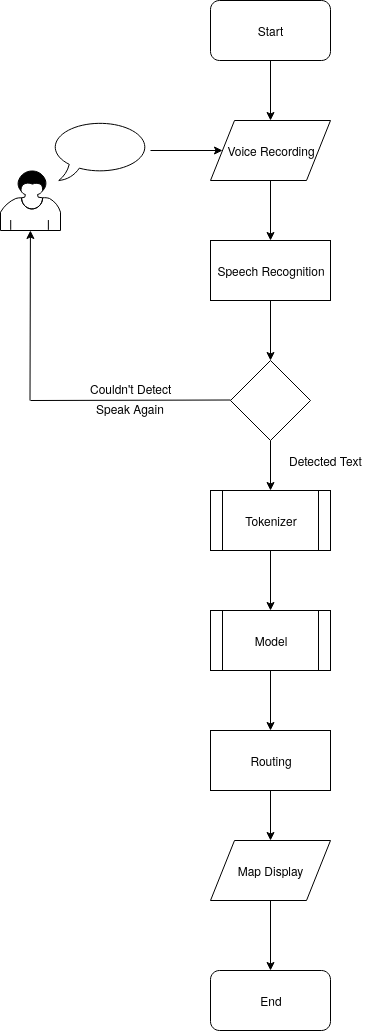
\includegraphics[scale=0.55]{flowchart}
    \caption{Flowchart of the Procedure}
\end{figure}
\vline